\documentclass[11pt, a4paper]{article}

\usepackage[left=2cm,text={17cm, 24cm},top=3cm]{geometry}
\usepackage[utf8]{inputenc}
\usepackage[czech]{babel}
\usepackage{times}
\usepackage{graphicx}
    \usepackage{float}
%    \usepackage{lscape}
    \usepackage{rotating}
%    \usepackage{showframe}
\usepackage{indentfirst}
\setlength\parindent{8pt}


\author{Jan Kubica, Juraj Korček}

\providecommand\ftnote[1]{\footnote{\raggedright#1}}

\usepackage{verbatimbox}
\raggedbottom

\begin{document}
	\begin{titlepage}
		\begin{center}
			\textsc{\Huge Vysoké učení technické v~Brně} \\[8pt]
			\textsc{\huge Fakulta informačních technologií} \\[16pt]
			\vspace{\stretch{0.382}}
			{\LARGE IDS - Databázové systémy} \\[6pt]
			{\huge Dokumentace k~projektu} \\
			\vspace{\stretch{0.075}}
			{\Huge \emph{Restaurace}} \\
			\vspace{\stretch{0.075}}
			{\Large 2016/2017}
			\vspace{\stretch{0.478}}
		\end{center}
		
		{\Large \hfill Juraj Korček (xkorce01)} \\[8pt]
		{\Large \today \hfill Jan Kubica (xkubic39)}
		
	\end{titlepage}


\section{Zadání}

   Vytvořte IS pro restaurační zařízení, který napomůže k~zjednodušení a zpřehlednění
jeho provozu. Restaurace je členěna do více místností a má přední a zadní zahrádku
a poskytuje běžné stravovací služby veřejnosti. Od informačního systému se požaduje,
aby, krom jiného, umožnil správu rezervací a objednávek. Rezervovat je možné jeden
nebo více stolů v~místnostech či na zahrádkách, anebo celé místnosti, případně i celou
restauraci pro různé společenské akce. Součástí rezervace také může být objednávka
nápojů a jídel. Systém musí umožňovat zaměstnancům restaurace vkládat objednávky
spolu s~informacemi, který zaměstnanec danou objednávku vložil a pro koho je určena.
Když se zákazníci rozhodnou zaplatit, musí jim systém vystavit účtenku. Po zaplacení
pak příslušný zaměstnanec vloží záznam o~platbě do systému. Systém by měl také
poskytovat podrobný přehled tržeb za vybrané období. Přístup k~této funkci bude mít
pouze majitel. V~neposlední řadě musí systém evidovat veškeré prodávané jídlo a pití
(včetně složení), přičemž majitel a odpovědný vedoucí mají možnost měnit ceny jídla
a pití nebo přidávat a odebírat položky.

\section{Návrh zpracování}

\subsection{ER diagram}

\begin{figure}[h]
    \centering
    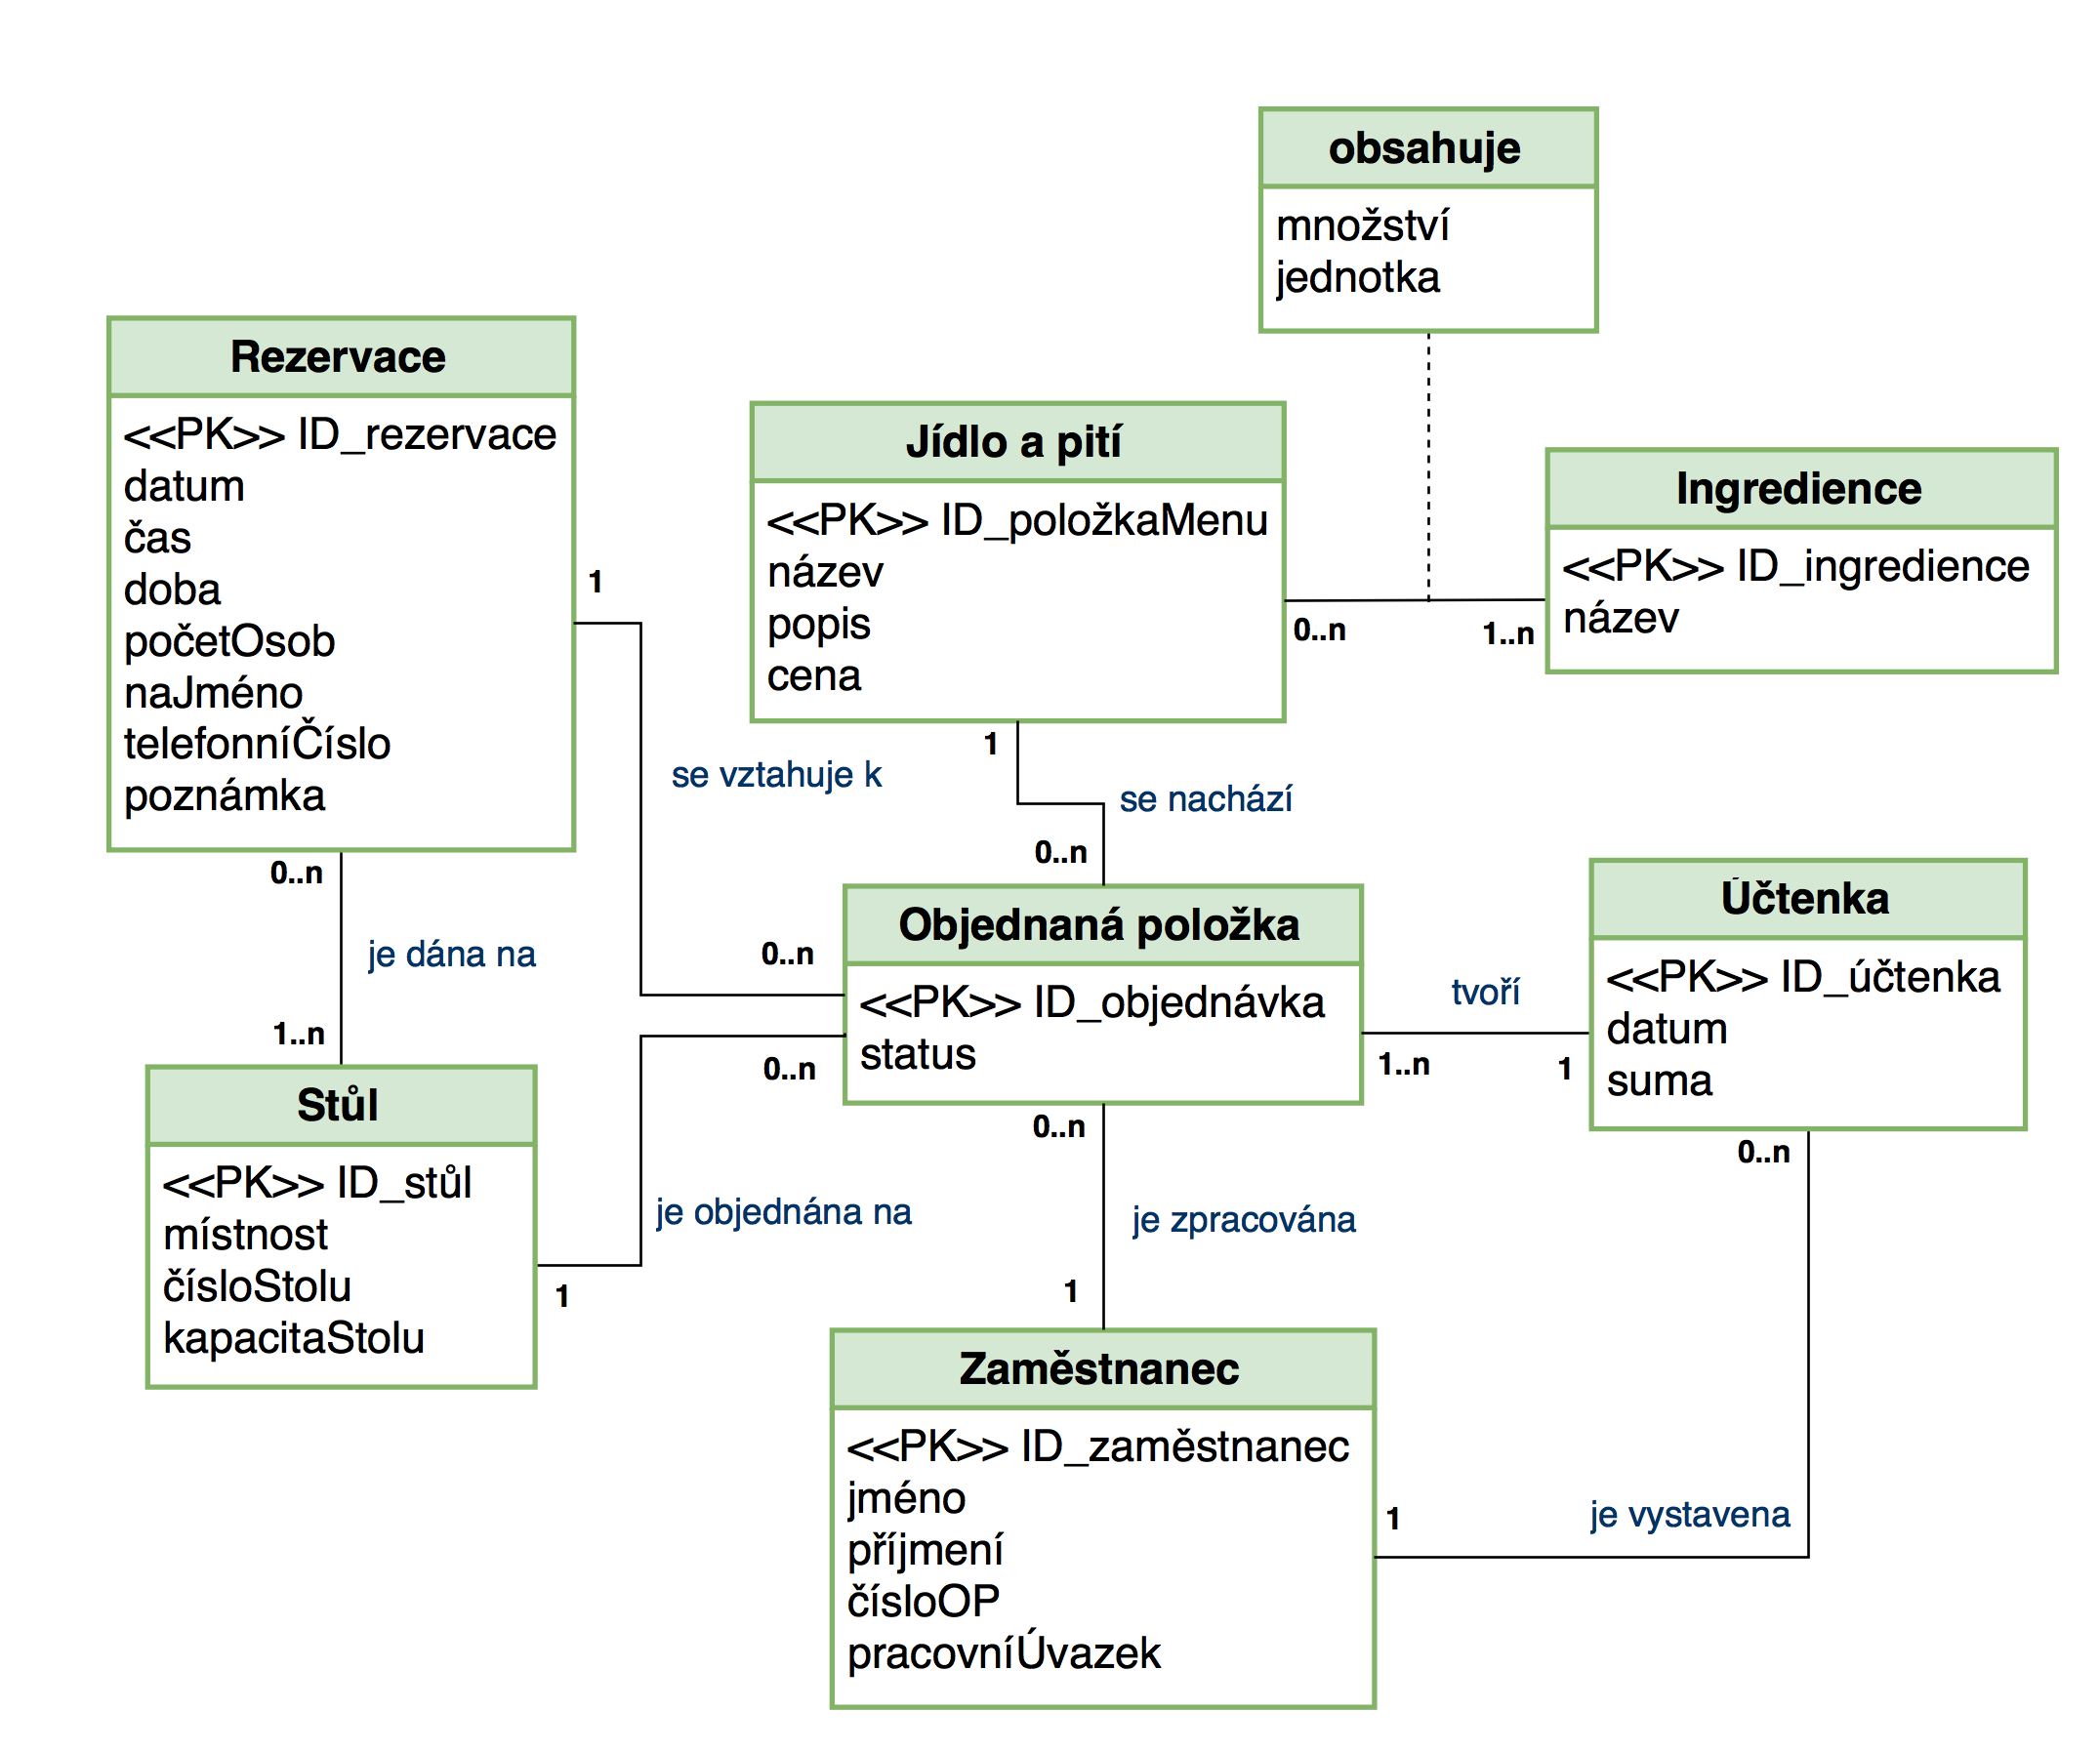
\includegraphics[width=42em]{ER}
    \caption{ER diagram}
 %   \label{ER diagram}
\end{figure}

% \begin{landscape}

\subsection{Schéma databáze}

\begin{figure}[H]
    \centering
    \rotatebox{90}{\includegraphics[width=0.90\textheight]{DS}}
    \caption{Schéma databáze generované v~Oracle SQL Developeru}
 %   \label{ER diagram}
\end{figure}

% \end{landscape}

\subsection{Generalizace/specializace}

 Realizaci vztahu generalizace/specializace jsme řešili spojením dvou entitních množin (jídla a pití) do jedné výsledné tabulky, přičemž byl přidán sloupec \textbf{\texttt{typ}} pro rozlišení dané kategorie. Tento sloupec pak nabývá pro každou položku menu buďto hodnoty \texttt{J} pro jídlo, anebo \texttt{P} pro pití. Pro ošetření správné jednotky byla přidána podmínka \texttt{CHECK}, která povoluje jídlu nastavit jednotku pouze z~množiny \{\emph{ g, kus }\}, pití pak \{\emph{ ml, cl, dcl, l }\}. K~tomuto řešení jsme přistoupili pro její snadnější a logičtější implementaci v~databázi.

\section{Implementace}

\subsection{Triggery}

V~rámci našeho řešení byly vytvořeny celkem tři triggery. Jako první např. \textbf{\texttt{TRG\_cena\_objednavka}}, který zajišťuje \emph{po vytvoření} objednané položky překopírování názvu a ceny z~tabulky \texttt{polozka\_menu} do tabulky \texttt{objednana\_polozka}. Takto jsme postupovali z~důvodu možnosti rychlejšího zpracování dotazů a taktéž kvůli obecně časté změně názvu či ceny položky menu v~budoucnu a následné integritě dat.

Jako druhý trigger byl implementován \textbf{\texttt{TRG\_status\_zaplaceno\_castka}}. Tento trigger se spouští \emph{po vytvoření} účtenky a umožňuje konkrétní označené objednané položky (status \texttt{oznaceno}) zaplatit (status \texttt{zaplaceno}), daným položkám pak přidělit cizí klíč na konkrétní účtenku a vypočítat celkovou sumu potřebnou pro právě vytvořenou účtenku.

Třetí trigger \textbf{\texttt{TRG\_cislo\_rezervace}} se spoutší \emph{před vytvořením} rezervace a nastavuje primární klíč ze sekvence složením aktuálního data a unikátního čísla v~rámci dne. Předpokládá se, že unikátní číslo by pak bylo pomocí procedury \texttt{reset\_seq} vynulováno každý den o~půlnoci.

\subsection{Procedury}

Procedura \textbf{\texttt{reset\_seq}} umožňuje resetování počítadla pro pořadí rezervace. Nejprve se načítá následující hodnota počítadla, která se poté od počítadla odečítá a tím se počítadlo inicializuje na nulu. Nakonec se určí minimální hodnota počítadla.

Procedura \textbf{\texttt{inc\_prices}} vykonává plošnou změnu cen danou procentem, které je předáno přes parametr. Procedura využívá explicitní kurzor, datové typy odkazující na sloupec tabulky a ošetření výjimek. Pokud uživatel zadá procento menší než -99\%, je na výstup vypsáno chybové hlášení.

Procedura \textbf{\texttt{spocti\_trzbu}} slouží k~vypočtení tržby v~určitém období daném dvěma daty předanými jako parametr. I~zde jsou využity datové typy odkazující na sloupec tabulky a také je ošetřena výjimka, kdy je v~prvním parametru zadáno pozdější datum než je datum v~druhém parametru.

%\subsection{Ukázkové výběry z dat databáze}
%- selecty

\subsection{Vytvoření indexu společně s~explain plan}

Pro optimalizaci byl vybrán následující SQL dotaz:

\begin{verbnobox}[\footnotesize]
SELECT nazev AS "Nazev jidla", COUNT(nazev) AS "Pocet ingrediencii"
FROM Polozka_menu NATURAL JOIN Obsahuje NATURAL JOIN Ingredience
WHERE typ = 'J'
GROUP BY nazev
ORDER BY COUNT(nazev) DESC;
\end{verbnobox}

\noindent
\newpage
%\\[-8pt]
Aby bylo možné určit cenu tohoto dotazu, byl použit \texttt{EXPLAIN\,PLAN},\ jehož výpis můžete vidět níže.

\begin{verbnobox}[\scriptsize]
---------------------------------------------------------------------------------------
| Id  | Operation             | Name           | Rows  | Bytes | Cost (%CPU)| Time     |
---------------------------------------------------------------------------------------                                 
|   0 | SELECT STATEMENT      |                |    24 |   888 |     6  (34)| 00:00:01 |                                
|   1 |  SORT ORDER BY        |                |    24 |   888 |     6  (34)| 00:00:01 |   
|   2 |   HASH GROUP BY       |                |    24 |   888 |     6  (34)| 00:00:01 |
|*  3 |    HASH JOIN          |                |    24 |   888 |     4   (0)| 00:00:01 |
|*  4 |     TABLE ACCESS FULL | POLOZKA_MENU   |     6 |   198 |     3   (0)| 00:00:01 |
|   5 |     INDEX FULL SCAN   | SYS_C001483240 |    24 |    96 |     1   (0)| 00:00:01 |
\end{verbnobox}
\noindent
\\[-8pt]
Jako prostředek pro urychlení byl vybrán index nad sloupcem \texttt{typ} tabulky \texttt{polozka\_menu}. Po aplikování indexu byl znovu použit \texttt{EXPLAIN PLAN}, který jasně demonstruje, že zavedení indexu optimalizovalo dotaz. Zde je možné vidět, jak se celková cena dotazu snížila a zatížení procesoru zvýšilo.

\begin{verbnobox}[\scriptsize]
-------------------------------------------------------------------------------------------------------
| Id  | Operation                               | Name         | Rows  | Bytes | Cost (%CPU)| Time     |
-------------------------------------------------------------------------------------------------------
|   0 | SELECT STATEMENT                        |              |    24 |   888 |     5  (40)| 00:00:01 |
|   1 |  SORT ORDER BY                          |              |    24 |   888 |     5  (40)| 00:00:01 |
|   2 |   HASH GROUP BY                         |              |    24 |   888 |     5  (40)| 00:00:01 |
|*  3 |    HASH JOIN                            |              |    24 |   888 |     3   (0)| 00:00:01 |
|   4 |     TABLE ACCESS BY INDEX ROWID BATCHED | POLOZKA_MENU |     6 |   198 |     2   (0)| 00:00:01 |
|*  5 |      INDEX RANGE SCAN                   | INDEX_TYP    |     6 |       |     1   (0)| 00:00:01 |
\end{verbnobox}

\subsection{Přístupové práva}

Přístupové práva pro druhého člena týmu byly definovány jako pro \emph{zaměstnance-číšníka}. \emph{Číšník} byl měl mít práva výběru, změny, vložení a mazání pro tabulky \textbf{\texttt{rezervace}}, \textbf{\texttt{stul}}, \textbf{\texttt{rezervace\_stul}}, \linebreak \textbf{\texttt{objednana\_polozka}}. Číšník by měl mít možnost výběru z~tabulky \textbf{\texttt{polozka\_menu}}, ale modifikovat ji může pouze provozní. Pro tabulku \textbf{\texttt{uctenka}} byly povoleny práva výběru, změny i vložení.

\subsection{Materializovaný pohled}

Pro druhého člena týmu byl vytvořen materializovaný pohled, který umožňuje \emph{práci s~rezervacemi}. Před vytvořením materializovaného pohledu musely být definovány přístupové práva pro tabulky patřící prvnímu členovi týmu. Kvůli optimalizaci byly vytvořené logy pro tabulky využívané materializovaným pohledem. Tyto logy umožňují zaznamenávat změny, a proto se nemusí při vložení dat procházet tabulka celá. Pro další optimalizaci byly při vytváření materializovaného pohledu použity operace: \texttt{REFRESH FAST ON COMMIT}, \texttt{ENABLE QUERY REWRITE} a \texttt{CACHE}.

\end{document}